\chapter{Conclusiones}

Al realizar los dos entrenamientos, uno con el agente local y otro con el global, se puede ver que el entrenamiento del local ha sido más preciso que su contraparte.

A continuacion, se pueden ver dos gráficas del agente local:
\begin{figure}[H]
    \centering
    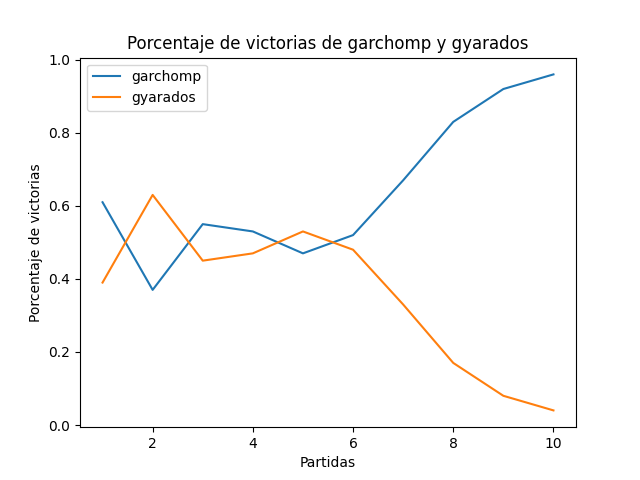
\includegraphics[width=0.7\textwidth]{figures/garchomp-vs-gyarados.png}
    \caption{Combate entre Garchomp y Gyarados.}
    \label{fig:turn}
\end{figure}

\begin{figure}[H]
    \centering
    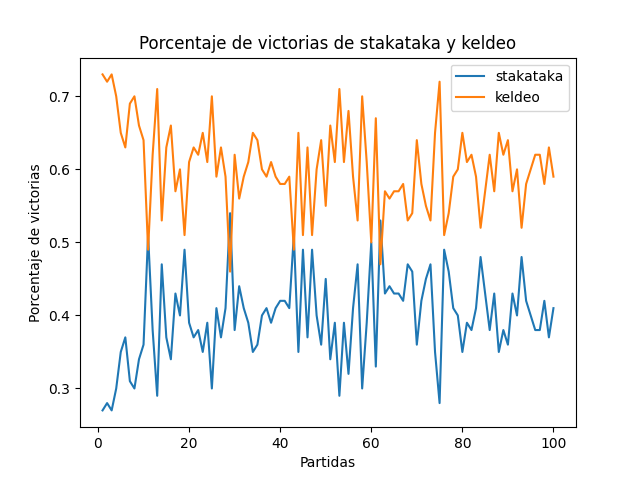
\includegraphics[width=0.7\textwidth]{figures/stakataka-vs-keldeo.png}
    \caption{Combate entre Stakataka y Keldeo.}
    \label{fig:turn}
\end{figure}

En ambas figuras se puede observar que la ia comienza eligiendo ataques de forma aleatoria hasta que encuentra uno que le permite ganar todas las partidas. De esta forma, se crea un balance entre ambos jugadores en el que uno gana siempre.

Hemos observado que al realizar el entrenamiento del agente global, existe un error que invierte el valor de las recompensas. Esto hace que el modelo tenga como objetivo perder. En la siguiente figura, la inteligencia artifial está jugando como el jugador 2, y vemos que solo tiene un porcentaje de victorias de aproximadamente 35%.

\begin{figure}[H]
    \centering
    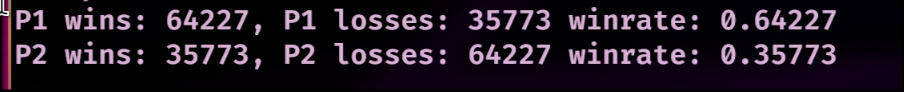
\includegraphics[width=0.9\textwidth]{figures/test_agente_global.jpeg}
    \caption{Combate entre Stakataka y Keldeo.}
    \label{fig:turn}
\end{figure}

\section{Posibles ampliaciones}

Además de solucionar el error presentado anteriormente, otras de las posibles mejoras para el proyecto incluyen utilizar más datos en el estado del juego, como por ejemplo las estadísticas de defensa y velocidad del pokémon. 

Una funcionalidad que no ha sido posible implementar es utilizar el motor gráfico del Pokémon Showdown para poder visualizar las batallas, e incluso probar los modelos contra jugadores reales online.
